%!TEX root = ../dokumentation.tex
\section{Analyse des Ist-Zustands}
Momentan werden unsere Djangoprojekte beim Commiten (Versionierung mit Hilfen von git) mit sognenannten ''pre-commit hooks'' analysiert. 
Dabei wird der Quellcode auf diverse Aspekte überprüft. Bei nicht bestehender Überprüfung wird eine Meldung ausgegeben.\\

\begin{center}
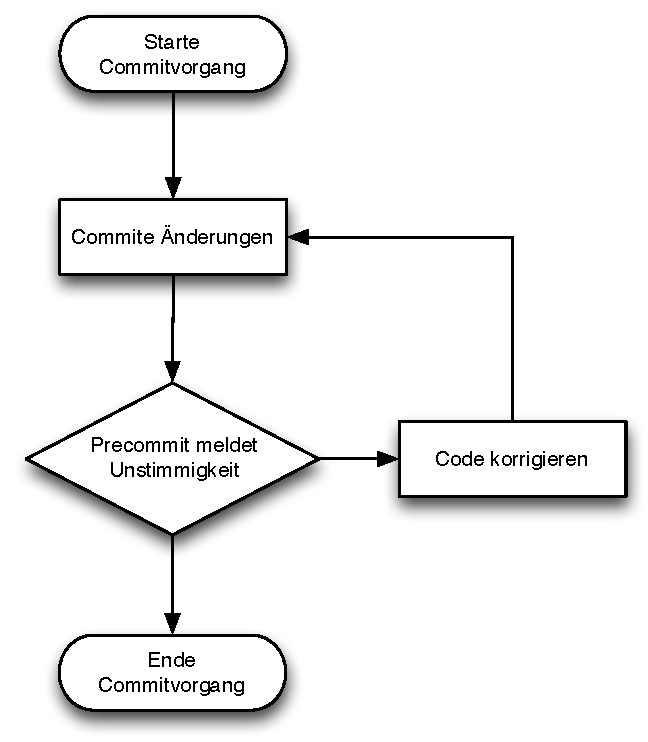
\includegraphics[width=0.6\textwidth,angle=0]{./grafiken/pzd_projektabarbeitung_ist.pdf}
\end{center}

Diese Methode hat bisher die Fehlerquate um einiges verringert. Es ist jedoch immer noch möglich einen Fehler in die Produktion einzuspielen. \\  
Folgende Ursachen können trotz pre-commit hooks einen Fehler auslösen. 
\begin{itemize}
    \item Man commited direkt über Github.
    \item Das requirements.txt für pip ist nicht vollständig.
    \item Programmierfehler, die nicht die Syntax betreffen. 
\end{itemize}
Derzeitig wird der Quellcode nach folgenden Zeichenkette überprüft:
\begin{itemize}
    \item ''import pdb'' - *.py: 
        pdb ist der Python Debugger. Aus Sicherheitsgründen darf dieser nicht in der Produktion verwendet werden.
    \item ''import ipdb'' - *.py:
        Gleiche Begründung wie ''import pdb''.
    \item ''print'' - *.py:
        Konsolenausgabe sind in der Produktion unerwünscht.
    \item ''console.log'' - *.js:
        Konsolenausgabe sind in der Produktion unerwünscht.
    \item ''debugger'' - *.js:
        Das Keyword ''debugger'' wird benötigt um Breakpoints zu setzen. Diese sind in der Produktion nicht erwünscht.
    \item 
\end{itemize}
Derzeitig wird der Quellcode mit folgenden tools überprüft:
\begin{itemize}
    \item jshint - *.js:
        jshint ist ein Code Qualitätstool, dass den Quellcode nach Fehlern und unschönen Programmiertechniken durchsucht.
    \item pyflakes - *.py:
        pyflakes überprüft den Quellcode nach potenziellen Fehlern.
    \item pep8 - *.py:
        pep8 ist ein Tool welches den Quellcode auf das Einhalten des pep8 Standards überprüft.
\end{itemize}

\subsection{Fehlererkennung}
Jede Djangoapplikation sendet im Fehlerfall automatisch ein Email an eine vorgebeben Email-Adresse mit einem ausführlichen Bericht. Darunter zählen jedoch nur Pythonfehler. Diese Funktionalität wird vom django Framework bereitgestellt. Wenn ein Fehler im settings.py auftritt, wird keine Fehlermeldung gesendet. Der Fehler bleibt unentdeckt bis jemand die Htmlseite aufruft. \\
Generell wird ein Fehler erst entdeckt wenn dieser ausgelöst wird. Das heisst, wenn ein Fehler nicht auf der lokalen Testumgebung ausgelöst und behoben werden kann, so wird mit zimmlicher Wahrscheinlichkeit der Besucher der Webapplikation den Fehler auslösen. \\
Fehler, die durch Serverprobleme verursacht werden, werden nicht speziel abgefangen oder kontrolliert, da diese relativ wenig vorkommen. 

\section{Gewünschter Soll-Zustand}
Die Probleme, die mit der jetztigen Qualitätssicherung auftreten sollen so weit wie möglich verhindert werden. Die meist auftretenden Fehler sollen weit weg vom Kunden entdeckt werden. Das heisst die Überprüfung müsste automatisiert und ständig auf einem externen System laufen.

\section{Ziele}
Für das erfolgreiche Abschliessen des Projekts müssen folgende Ziele erfüllt sein:
\begin{itemize}
    \item Es wird täglich sichergestellt, dass der Pythoncode einer definierten Anzahl von Kriterien enspricht. 
          Darunter gehören sowohl Syntax wie auch Codedarstellung.
    \item Es wird täglich sichergestellt, dass jedes Projekt sammt Abhängikeiten ordnungsgemäss installiert und wieder deinstalliert werden kann.
    \item Man kann ohne Änderungen am Basecode weiter Prüfungsanwendunge dem Script hinzufügen. 
    \item Es kann eine belibige Anzahl von Projekte überprüft werden.
\end{itemize}
\clearpage
